%!TEX root = main_arduino_intro.tex

\chapter{Sample cooling stage}\label{chap:sample_cooling_stage}

Over the last few chapters, we have slowly gone through all the individual components that we need in order to assemble a complete sample cooling stage with feedback control. Let us now take this knowledge and assemble the whole project. Figure~\ref{fig:complete_setup:breadboard_setup} shows an image of a complete setup. 
\begin{figure}[tb]
    \centering
    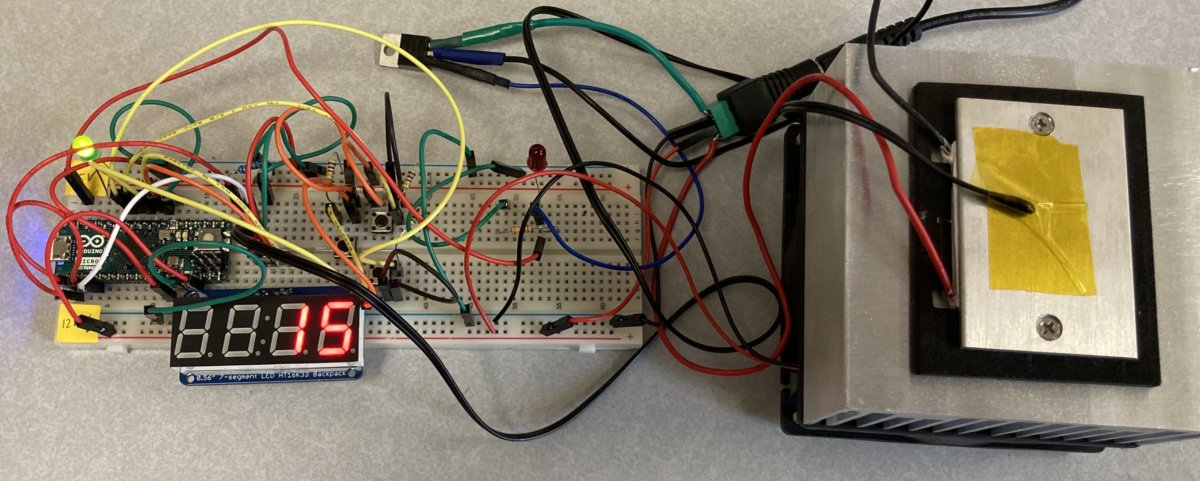
\includegraphics[width=0.8\textwidth]{graphics/05_complete_setup/full_setup_breadboard.jpg}
    \caption{Complete setup of the sample cooling stage, set to 15\celsius.}
    \label{fig:complete_setup:breadboard_setup}
\end{figure}
In the end, our setup should be able to do the following:
\begin{itemize}
    \item Run independent of a computer
    \item Have two \acp{led}: A green one indicating that the thermocouple is within the specified temperature range and a red \ac{led} showing the \ac{pwm} output to the \ac{mosfet} that drives the cooler
    \item A display showing the current temperature or the set temperature, depending on the mode the device is in
    \item Buttons to enter / exit the set mode and additional buttons to increase / decrease the set temperature
    \item \ac{mosfet} \ac{pwm} control to drive the thermoelectric cooler
\end{itemize}

\infobox{Breadboard power busses}{We use 5\,V and 12\,V power for various components. It is recommended that you wire both power buses on the breadboard, one with 5\,V from the Arduino and one with 12\,V from the \ac{dc} power supply. For the 12\,V bus: Be careful to ground it through the \ac{dc} power supply and do not connect any Arduino pin other than the \texttt{VIN} and ground pins (see Figure~\ref{app:pinout}). Before you connect even these pins, read Section~\ref{sec:complete_setup:vin}.}

The following sketch gives one potential setup for implementing the full controller. A template Arduino \texttt{ino} file with this content can be found on \href{https://github.com/galactic-forensics/workshop_arduino_electronics/blob/main/templates/full_project_template/full_project_template.ino}{GitHub}.

\begin{lstlisting}
// Load libraries
// Adafruit Display initialization
// Variables and Pins for temperature measurement
// Variables for set temperature
// Thermoelectric cooler variables and Pins
// Button pins to set temperature
// LED Pins and temperature happiness range

void setup() {
  // Initialize Adafruit display
  // Initialize pin modes for buttons, PWM for cooler, LEDs
}

void getTemperature() {
  // Read thermistor, calculate and store temperature
}

void setDisplay(int valueToSet, bool setpoint=false) {
  // Set the display with a value to set (integer)
  // Additionaly display 'S' if we are in set mode
}

void setMode() {
  // Check if we are in set mode and adjust display
  // If in set mode, adjust set point if called for
}

void controlTEC() {
  // Control the termoelectric cooler.
}

void checkTemperatureOk() {
  // If temperature in given range, turn green LED on
}

void loop() {
  // Your main loop to hang everything together
}
\end{lstlisting}
In the following chapters, we will slowly expand this template until the controller  is working. For all the individual subroutines you should already have existing code from the previous exercises. Recycle your code when adequate! You can also initialize the serial console in order to print to the screen when necessary. Note that the following chapters all build on the above template and on each other.

\section{Read the temperature}

As a first step, we want to read the resistance of the thermocouple and then transform the read value into a temperature in \celsius. You should already be familiar with this task from Chapter~\ref{chap:temperature}. Make sure that your temperature reading is stable, i.e., average a few measurements for the best results.

\exerbox{Define an overall global variable \texttt{currentTemperature}. Then re-use your previous code and put it into \lstinline{void getTemperature() \{...\}} such that this subroutine, when called, writes the current temperature to the variable you just defined. Then read the current temperature and print it to the serial console from the main loop.}


\section{Integrate the display}

In the next step, we will integrate the display. Make sure that you load the required Adafruit libraries. You have already controlled the display in Chapter~\ref{chap:display}. You can integrate a way to display the set point already, however, we won't use this integration for now.

\exerbox{Integrate the display. Re-use your previous routine to display the current temperature in steps of whole degrees. You should also allow the \lstinline{void setDisplay (int valueToSet, bool setpoint=false)\{...\}} to take two variables, the temperature as an integer to directly display it and a boolean variable. If this boolean is \lstinline{true}, the display should write an s (a \lstinline{5}) into the first digit to indicate that we are in set mode (see next Section). After reading the temperature in the main loop, display it on the display. 

Hint: It might be useful to round the temperature before displaying the floating point number as an integer. Otherwise, the displayed temperature will be rounded incorrectly when it is high, since \cpp\ simply cuts off everything after the decimal point when converting a \lstinline{float} to an \lstinline{int}.}

\section{Set mode for the temperature}

Since we want to use our setup independent of a computer, we want to allow the user to change the set temperature. You can use various interfaces for this. I am using a three button setup. The buttons do the following:
\begin{itemize}
    \item \lstinline{setModeButton}: Enter / exit (toggle) the set-mode
    \item \lstinline{plusButton}: Increase the temperature if in set mode
    \item \lstinline{minusButton}: Decrease the temperature if in set mode
\end{itemize}
Furthermore, you should also set reasonable upper and lower limits that the user cannot exceed. Such limits could, e.g., be 25\celsius for the upper level (approximately room temperature) and -10\celsius for the lower level. Think of these levels as limits to prevent the user from setting insane, unreachable set points.

\exerbox{Implement the set mode. Pressing the \lstinline{setModeButton} should toggle a boolean that allows you to decide if the set mode is on or not. 
If the set mode is on, the display should display the setpoint temperature. Pressing this button again will deactivate the set mode and display the current temperature again. 

If in set mode, the plus and minus buttons should in- and decrase the set point, respectively. Check for button presses in the \lstinline{void setMode() \{...\}} routine. Make sure that the button presses cannot happen too fast, e.g., include a delay after each press to allow for user interaction time (typically a few hundred milliseconds).}


\section{Thermoelectric cooler}

Now that we have the set mode as well as the temperature reading established, we can implement the thermoelectric cooler. As a first step, we won't go into control theory and use simple on/off logic. The next chapter outlines further and fancier implementations of this control. Therefore, make sure that you already connect the cooler control to an \ac{io} pin that is capable of \ac{pwm} output. For now, we will simply turn the cooler on if the temperature set point is below the actual temperature, and turn it off otherwise.

\exerbox{Implement the thermoelectric cooler to turn it on and off, depending on the setpoint and current temperature comparison (see above). Implement this comparison in the \lstinline{void controlTEC() \{...\}} subroutine and call this subroutine from your main loop. Connect a red \ac{led} to the \ac{mosfet} control pin, this \ac{led} will then tell you if the cooler is on or off.}


\section{Status \ac{led}}

Finally, we are going to incorporate a green \ac{led} that will allow us to see at once if the system is at temperature or not. Let us, e.g., define a temperature range of $\pm0.5$\celsius in which we would call the achieved temperature acceptable. 

\exerbox{Set up a green \ac{led}. This \ac{led} will be controlled in the routine \lstinline{void checkTemperatureOk() \{...\}}. In this routine, compare the current temperature to the set point and turn the \ac{led} on when you are inside your defined happiness zone, otherwise turn it off. Note: the function \lstinline{abs()} might come in handy: it takes the absolute value of a given number.}


\section{Run independent of a computer}\label{sec:complete_setup:vin}

So far, we have always powered the Arduino from the 5\,V that come from the USB connection from the computer. However, most boards also have a \texttt{VIN} pin. This allows us to connect an external power source and not use the computer at all.
The recommended voltage on the \texttt{VIN} pin is 7-12\,V and the maximum voltage 6-20\,V. 

Since we have a 12\,V power supply to drive the thermoelectric cooler, we can use the same power source to drive the Arduino. Since we are using a 5\,A power supply, we won't have the full current that can be used by the cooler anymore, however, the Arduino only uses very little power, so this should not matter too much. Otherwise, we could always replace the power supply with one that has a higher current rating.

\exerbox{Connect an Arduino ground pin to ground (the negative side of the 12\,V supply) and the \texttt{VIN} pin to the 12\,V. Be careful not to mix up the pins, you might destroy your Arduino otherwise! Your setup should run now without a computer connection. If you need to restart the Arduino for any reason, you can use the reset button that is onboard.}


\section{Testing}\label{sec:complete_setup:testing}

If all went well, your setup might look similar to the one shown in Figure~\ref{fig:temperature:final_setup}. Congratulations!

Finally, before you want to use your temperature controller, you might want to test it for stability. Does it really fulfill your requirements or do you need to adjust the capabilities? Some test ideas are outlined in the following list:
\begin{itemize}
    \item How stable is your set temperature over the long run?  Does the green \ac{led} stay lit once it reaches the desired temperature?
    \item How about changing the ``load''? Put a glass of water on the cooler and submerge the thermistor to measure the water temperature. You have now added a ballast. Does the temperature stay constant once the set point is reached?
    \item Narrow the temperature range that you decide is acceptable and check if your setup can hold this narrower range
    \item Interface test: Give the device to a friend and check if the interface is intuitive
    \item Is your setup feasible / can it be used in a production scenario?
\end{itemize}

For many of these tests you might actually realize that your setup still needs improvements. These improvements are likely in design, setup, and integration of the cooling control. The next chapter gives you an outlook on where to go from here, i.e., what else you might want to think about if you really want to use this setup in your lab.